\documentclass[tikz,border=2pt]{standalone}
\usepackage{amsmath}
\usetikzlibrary{arrows.meta}
\begin{document}
% Pizza stand (Exercise 5.2.8): lambda(0..4) = 10,10,20,20,5 per hour, mu(1) = 30, mu(n) = 60 for n >= 2.
% q(n+1) = q(n) lambda(n)/mu(n+1) from q(0) = 1; G = sum q(n) = 1.4141; p(n) = q(n)/G.
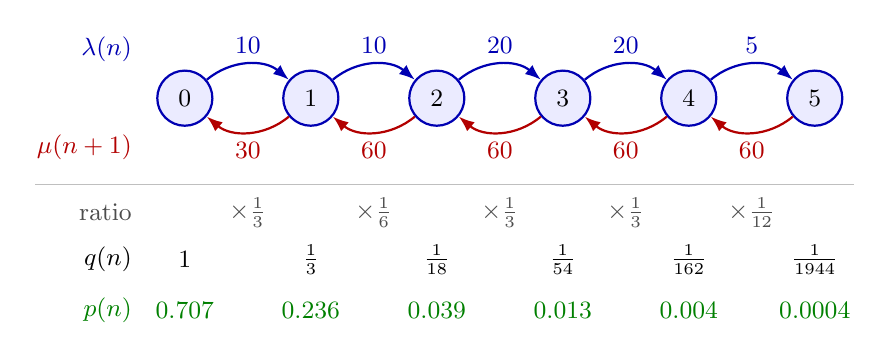
\begin{tikzpicture}[font=\small, >={Latex[length=2mm]},
  st/.style={circle, draw=blue!70!black, thick, fill=blue!8, minimum size=7mm, inner sep=0pt}]
  \def\d{1.6}
  \foreach \n in {0,...,5} \node[st] (s\n) at (\d*\n,0) {$\n$};
  % arrival rates (up) and service rates (down)
  \foreach \n/\m/\l in {0/1/10,1/2/10,2/3/20,3/4/20,4/5/5}
    \draw[->, thick, blue!70!black] (s\n) to[bend left=40] node[above] {$\l$} (s\m);
  \foreach \n/\m/\l in {0/1/30,1/2/60,2/3/60,3/4/60,4/5/60}
    \draw[->, thick, red!70!black] (s\m) to[bend left=40] node[below] {$\l$} (s\n);
  \node[blue!70!black, anchor=east] at (-0.55,0.62) {$\lambda(n)$};
  \node[red!70!black, anchor=east] at (-0.55,-0.62) {$\mu(n+1)$};
  % step ratios
  \foreach \n/\r in {0/3,1/6,2/3,3/3,4/12}
    \node[gray!60!black] at (\d*\n+0.5*\d,-1.45) {$\times\tfrac{1}{\r}$};
  \node[gray!60!black, anchor=east] at (-0.55,-1.45) {ratio};
  % unnormalized weights
  \foreach \n/\q in {0/1,1/\tfrac{1}{3},2/\tfrac{1}{18},3/\tfrac{1}{54},4/\tfrac{1}{162},5/\tfrac{1}{1944}}
    \node at (\d*\n,-2.05) {$\q$};
  \node[anchor=east] at (-0.55,-2.05) {$q(n)$};
  % normalized probabilities
  \foreach \n/\p in {0/0.707,1/0.236,2/0.039,3/0.013,4/0.004,5/0.0004}
    \node[green!50!black] at (\d*\n,-2.7) {$\p$};
  \node[green!50!black, anchor=east] at (-0.55,-2.7) {$p(n)$};
  \draw[gray!50, thin] (-1.9,-1.1) -- (5*\d+0.5,-1.1);
\end{tikzpicture}
\end{document}
